
\documentclass{article} % Don't change this

\usepackage[english]{babel}
\usepackage[utf8]{inputenc}
\usepackage[margin=1.2in]{geometry}
\usepackage{amsmath}
\usepackage{amsthm}
\usepackage{amsfonts}
\usepackage{multirow}
\usepackage{amssymb}
\usepackage{multicol}
\usepackage{booktabs}
\usepackage[usenames,dvipsnames]{xcolor}
\usepackage{graphicx}
\usepackage[siunitx]{circuitikz}
\usepackage{tikz}
\usepackage{lscape}
\usepackage[colorinlistoftodos, color=orange!50]{todonotes}
\usepackage{hyperref}
\usepackage[authoryear]{natbib}
\setcitestyle{authoryear,open={(},close={)}}
\usepackage{fancybox}
\usepackage{epsfig}
\usepackage{soul}
\usepackage{listings}
\usepackage{subcaption}
\lstset{language=[90]Fortran,
  basicstyle=\ttfamily,
  keywordstyle=\color{red},
  commentstyle=\color{green},
  morecomment=[l]{!\ }% Comment only with space after !
}

\usepackage{booktabs}
\setlength{\marginparwidth}{3.4cm}

%#########################################################

%To use symbols for footnotes
\renewcommand*{\thefootnote}{\fnsymbol{footnote}}
\newcommand{\tp}{\texttt}
%To change footnotes back to numbers uncomment the following line
%\renewcommand*{\thefootnote}{\arabic{footnote}}

% Enable this command to adjust line spacing for inline math equations.
% \everymath{\displaystyle}

\title{\raggedright
\normalfont \normalsize 
\huge Multi-threaded Programming: Scheduling and Affinity Coursework \\[1em]
\normalsize \normalfont Jack Tyler: 27513556 \\
\rule{\linewidth}{.5pt}  \\[6pt]
}

\begin{document}

\maketitle

In the early days of computing, computational power progressed at an alarming rate; constant field scaling meant that transistors could be fabricated smaller and smaller, allowing them to use less power, and to increase their clock speed.
However, transistor manufacture has hit a physical limit for scaling \citep{Mcfarland1995}, and increasing the clock speed any further would require highly capable cooling solutions impractical for use.
As a result, processor companies have had to find other methods to speed up computer processor to keep computational power, and Moore's Law, advancing.
Perhaps most prominent is the introduction of parallelism, where multiple processor units may exist on a processor `chip', and execute asynchronously and independently.

This type of parallelism is one of the most common implementations currently used in high-performance computing to decrease program execution time.
However, care must be taken as to how each processor unit -- each thread -- is synchronised to complete a computational task in unison. In particular,
some methods of synchronisation, or scheduling, may provide better performance for a particular application.

This report investigates the most effective scheduling algorithm for a particular computational problem on the ARCHER supercomputing cluster.
In particular, it studies the effectiveness of scheduling algorithms provided by the OpenMP standard, compared to a static partitioned affinity schedule work-stealing algorithm specifically designed for the computation problem at hand, and identifies many of the limitations and shortcomings in both the paralellisation of the algorithm, and in the analysis method. Knowledge of the OpenMP standard and parallel computing nomenclature is assumed in this report.

\section*{Scheduling algorithms}

Scheduling algorithms determine the distribution and synchronisation of work to the threads on the processor.
It's possible to quantify a scheduling algorithm's performance based on its effectiveness in minimising four separate overheads:
synchronisation, where threads must idle to wait for another thread to finish some task;
communication, where interactions between processors do not proceed optimally, such as cache misses and non-local memory accesses;
worker initialisation, where time is requried to initialise, schedule and destroy pools of parallel workers;
and load imbalances, where some threads are idle while others are still performing work.
The latter is perhaps the most important for this runtime optimisation, since the loops studied here are relatively poorly balanced.
Indeed, a major metric used in this thread is the amount of time threads would spend idling.

We may define two distinct types of self-scheduling algorithms: fixed, and variable.

In fixed systems, each processor will be assigned a fixed amount of work at loop initialisation, and continue computing until all their assigned work is completed.
While this can reduce scheduling overhead, in potentially only distributing and synchronising once, this method can be inappropriate for imbalanced loops, since some loops may idle unnecessarily while other threads are still working, providing a bottleneck on execution times.
Indeed, profiling the programs used later in the report shows that OpenMP scheduling overheads are up to 6\% of program execution time.

In the OpenMP standard, we may also specify the chunk size -- that is, the number of iterations assigned to each thread -- which can adjust scheduling performance depending on our load balancing.
Small chunk sizes will incur large schediling overheads, but will be able to smooth out load imbalances by constantly reassigning work, regardless of other threads being busy.
Similarly, large chunk sizes will reduce scheduling overheads, but amplify and load imbalances.

Variable algorithms will adjust their chunk sizes as the loop progresses. 
In the OpenMP standard, two such algorithms exist: \tp{DYNAMIC} and \tp{GUIDED}.
\tp{DYNAMIC} functions by assigning variable chunk sizes to threads, and working on a `first-come, first-served' basis.
This works well for imbalanced loops, since work can be reassigned when threads would otherwise be idling, at the cost of scheduling overheads.

\begin{figure}
    \begin{lstlisting}
        do i = 1,N

            do j = N,i,-1
        
                a(j,i) = a(j,i) + cos(b(j,i))
        
            end do
      
        end do
    \end{lstlisting}
    \caption{Loop 1; note that this loop is well-balanced, and we should expect each thread to perform approximately the same amount of work for this loop.}
    \label{listing:loop1}
\end{figure}

\tp{GUIDED} functions similarly, but by assigning initially large numbers of iterations and then getting exponentially smaller.
By doing so, the scheduling overheads are kept relatively small -- with the large chunk assignments at the beginning -- but the possibility for good load balancing is still present at the end of the iterations, when small chunks are used.

Most compilers will also support an \tp{AUTO} option, which lets the compiler determine the scheduling to implement (be it OpenMP-standard or otherwise).
However, there is no transparency in the scheduling implemented here, although there is the possibility of the scheduling changing to reflect observed behaviour with some compilers.

\section*{Introduction to the Problem}

The problem statement for this work is, at first glance, straightforward: to parallelise two exemplar computation loops, and to investigate the effect of OpenMP-standard scheduling algorithms, or indeed a third-party algorithm, on program run-time.
However, it's worthwhile to first understand and consider potential approaches and pitfalls that may be experienced from an examination of the loop structures.

Loop 1 (Figure \ref{listing:loop1}) is a simple, yet relatively imbalanced nested do-loop; each repetition of the inner do-loop is variable based on the value of \texttt{i}.
As a result, threads that are assigned a different value of \tp{i} will perform a different amount of work (Figure \ref{fig:loop1work}).
We might therefore expect scheduling algorithms that work well with a slight work imbalance to perform well on this problem, such as \tp{GUIDED,\textit{n}}, or \tp{DYNAMIC,\textit{n}}. 
However, since the distribution of work is readily predictable, we may see good performance from the \tp{AUTO} option, which gives the compiler the authority to change the scheduling algorithm as it sees fit (including during runtime).

\begin{figure}
    \centering
    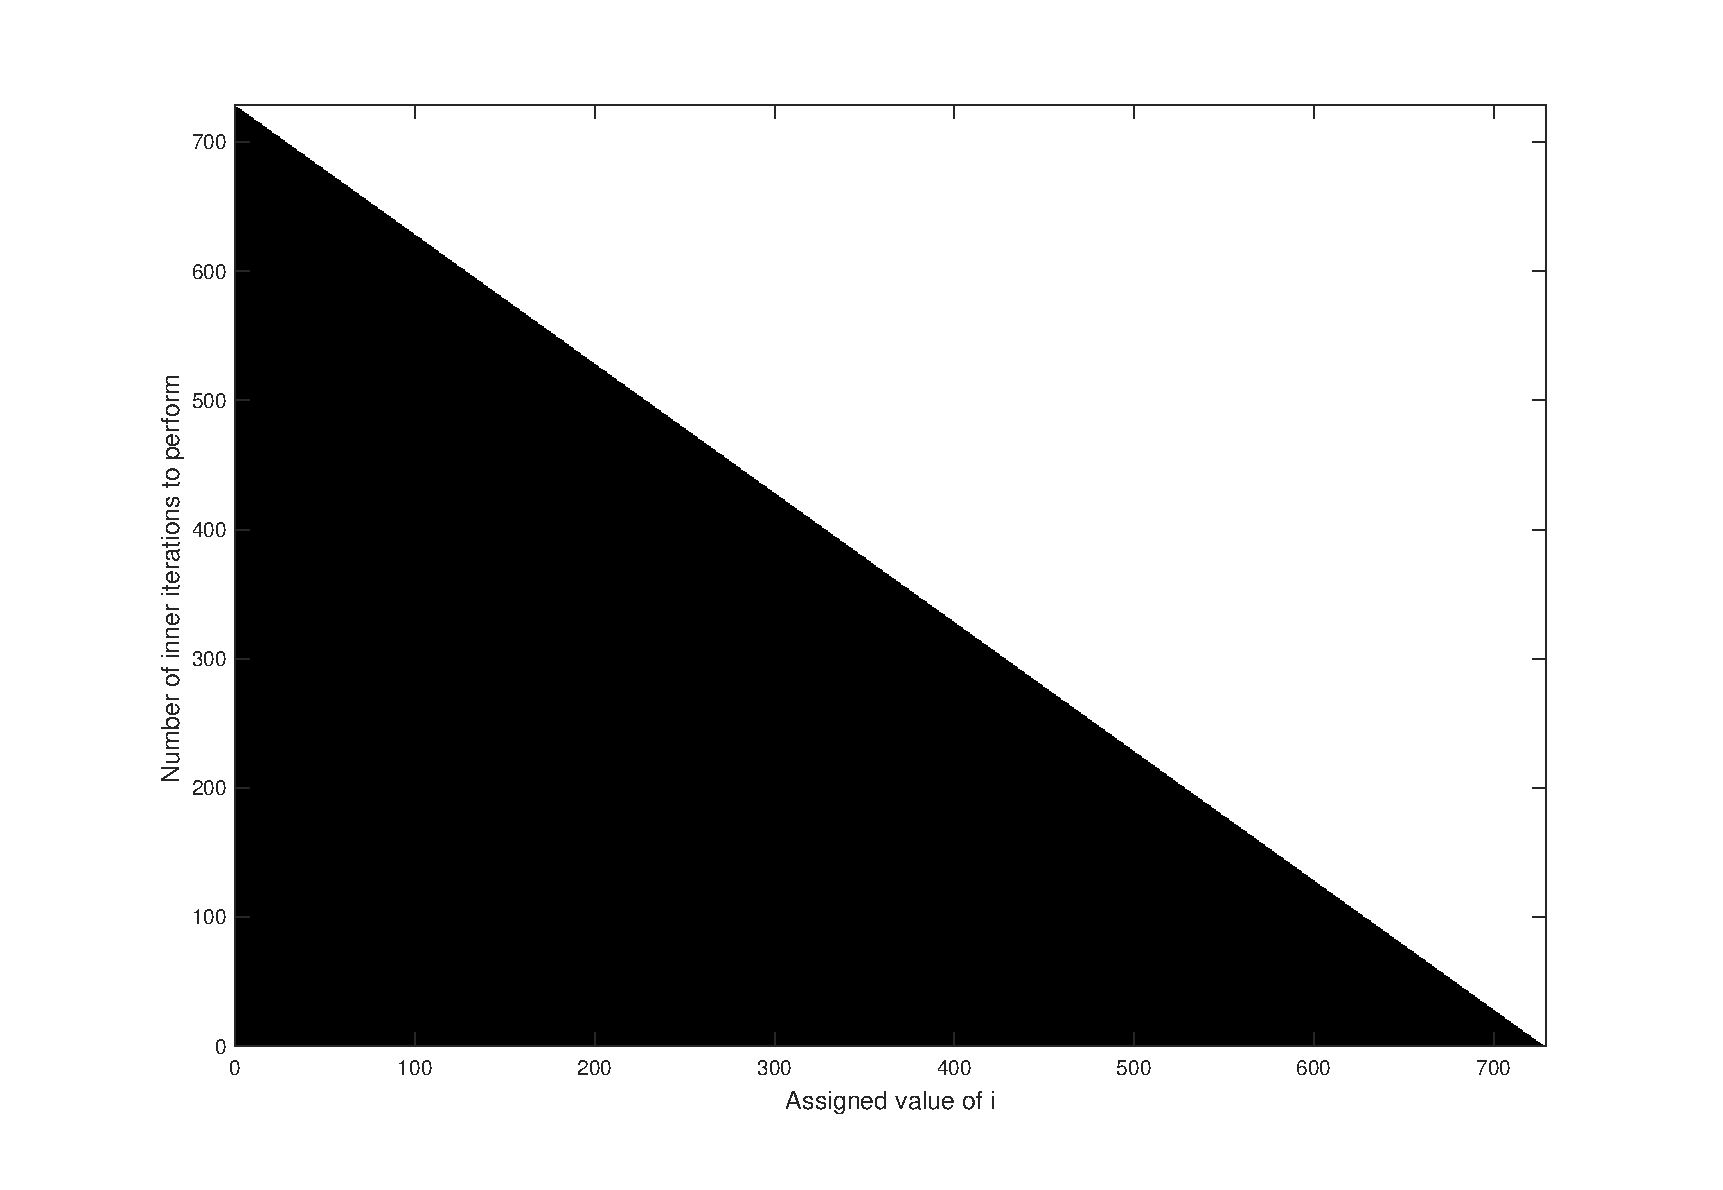
\includegraphics[height=.3\textheight]{part1_plots/loop1_balancing.eps}
    \caption{The number of inner-loop iterations in Loop 1 a thread must perform based on the value of \tp{i} it is assigned; while this is a slight work imbalance, the number of iterations to perform is readily predictable.}
    \label{fig:loop1work}
\end{figure}
    
\begin{figure}
    \centering
        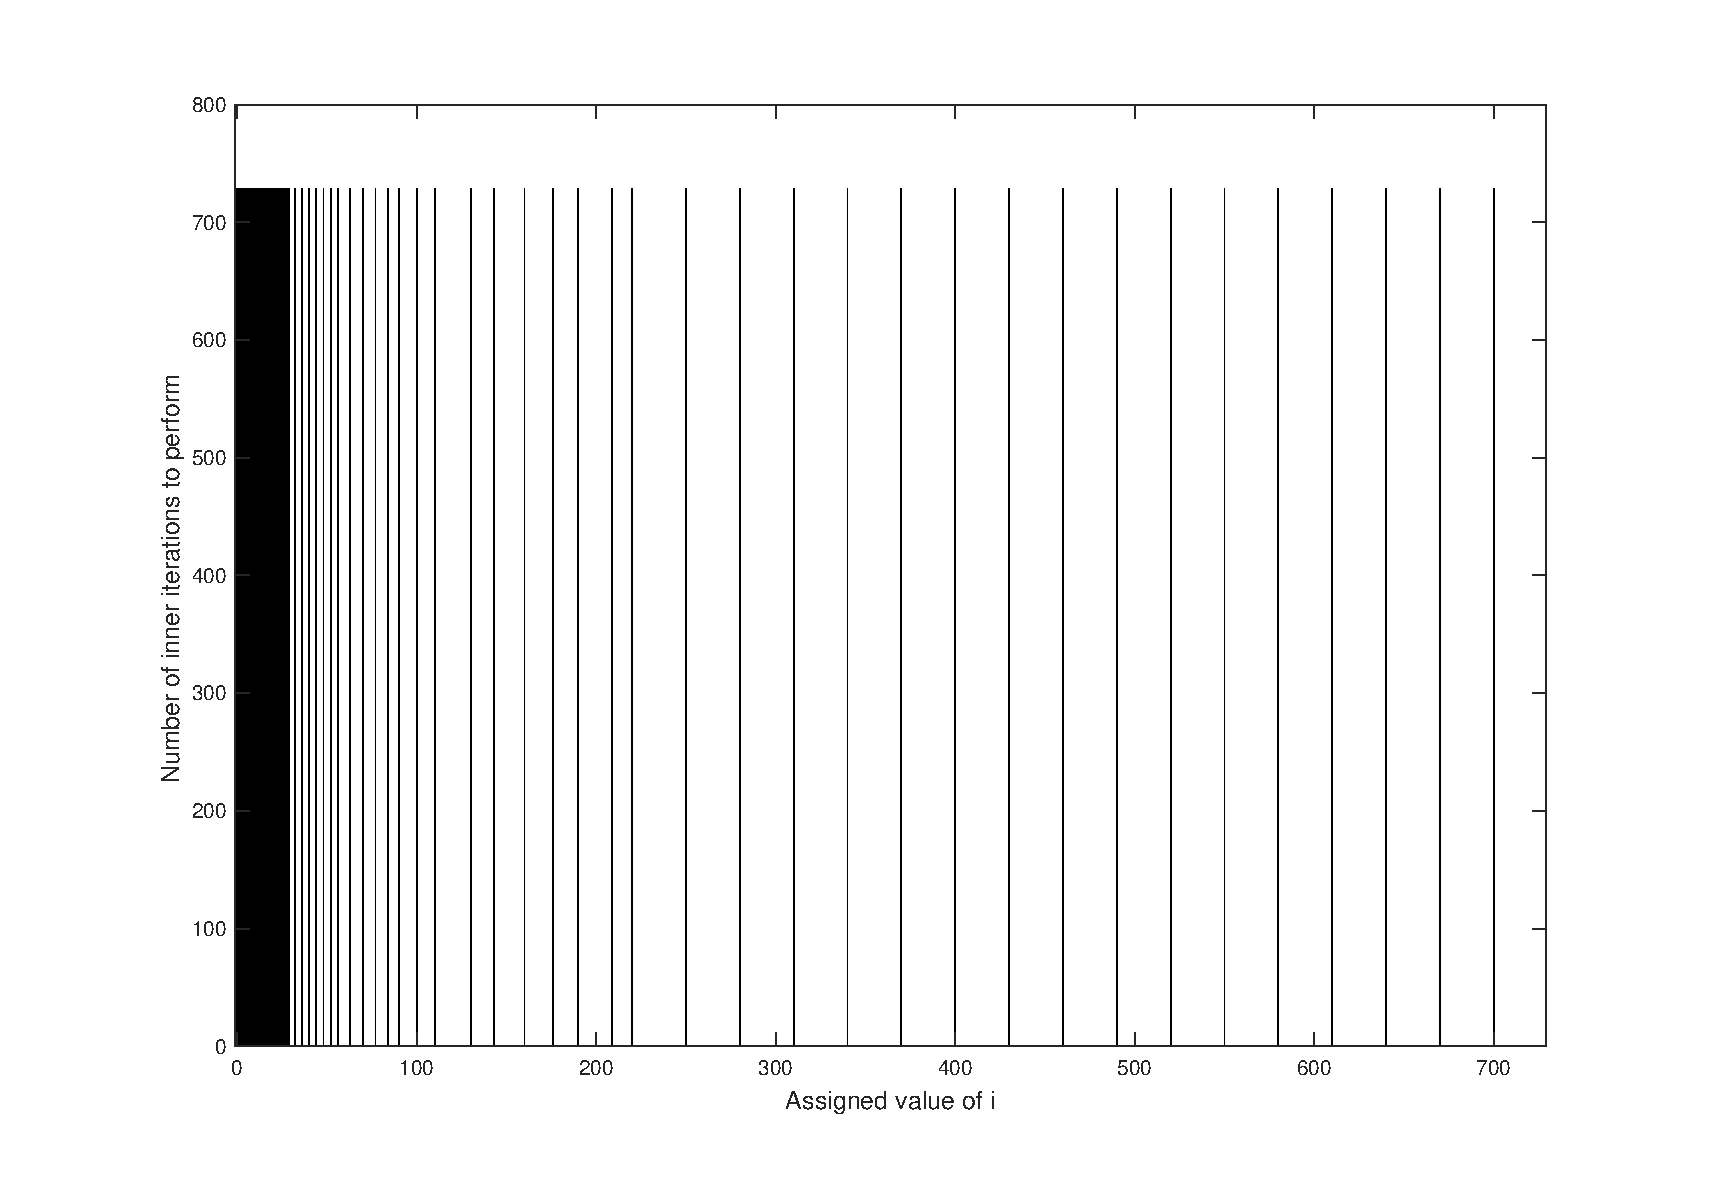
\includegraphics[height=.3\textheight]{part1_plots/loop2_balancing.eps}
        \caption{The number of inner-loop iterations in Loop 2 a thread must perform based on the value of \tp{i} it is assigned; note that threads may be required to perform either $1$ or $729$ inner iterations. This is a severe work imbalance that would need to be addressed effectively to maximise performance.}
        \label{fig:loop2work}
\end{figure}

Loop 2 (Figure \ref{listing:loop2}) is a poorly-balanced loop.
The \texttt{i}-th element of \texttt{jmax} is initialised to either $1$ or $N$, depending on the value of \texttt{i}.
As a result, a thread which is assigned the work of a value of \texttt{i} equal to $N$ will perform far more work than the threads with only $1$ inner iteration (Figure \ref{fig:loop2work}).
Loop scheduling algorithms that are suitable for loops with widely fluctuating work levels, such as \tp{DYNAMIC} or \tp{GUIDED}, would be expected to work well here.
More specifically, since the majority of work is scheduled in the first 30 iterations, and approximately every 30 iterations thereafter, performance may be best for chunk sizes less than 30.
The work repeated every 30 iterations will also prevent threads from becoming idle and accepting more work.

\section*{OpenMP-standard Scheduling: Varying chunk sizes}

\subsection*{Implementation}

Loop 1 and Loop 2 represent `embarassingly parallel' problems, and as such, parallelising the routines was relatively trivial: both loops were enclosed in a \tp{!\$OMP PARALLEL DO} construct, and set such that their arrays were shared (as well as \tp{rN2} in the case of Loop 2), with all other variables set private.
The scheduling algorithm was then set to be allocated at runtime -- \tp{SCHEDULE(RUNTIME)} -- and the associated \tp{OMP\_RUNTIME} environment variable was exported to the compute node at job submission, which was controlled by a lightweight governing bash script that would parametrically generate the PBS submission file for every possible combination of scheduling algorithm and chunk size.
The program was designed to take in the number of threads to use as a command line argument to the program execution.
The results of an \tp{OMP\_GET\_SCHEDULE} call as part of the main Fortran program were printed to the screen to ensure the correct scheduling algorithms; the call returns integers of type \tp{omp\_schedule\_kind} that can be cross-checked against the scheduling kinds contained in the \tp{omp\_lib\_kinds} module as part of \tp{libgomp}.

Submitting all of the jobs as a batch also meant that the timing results were more accurate, as jobs were almost-guaranteed to be computed on the same node.
Each job was repeated five times, and an average taken, to remove the effects of variable computational performance on each run.

\subsection*{Results}

% \begin{figure}
%     \centering
%     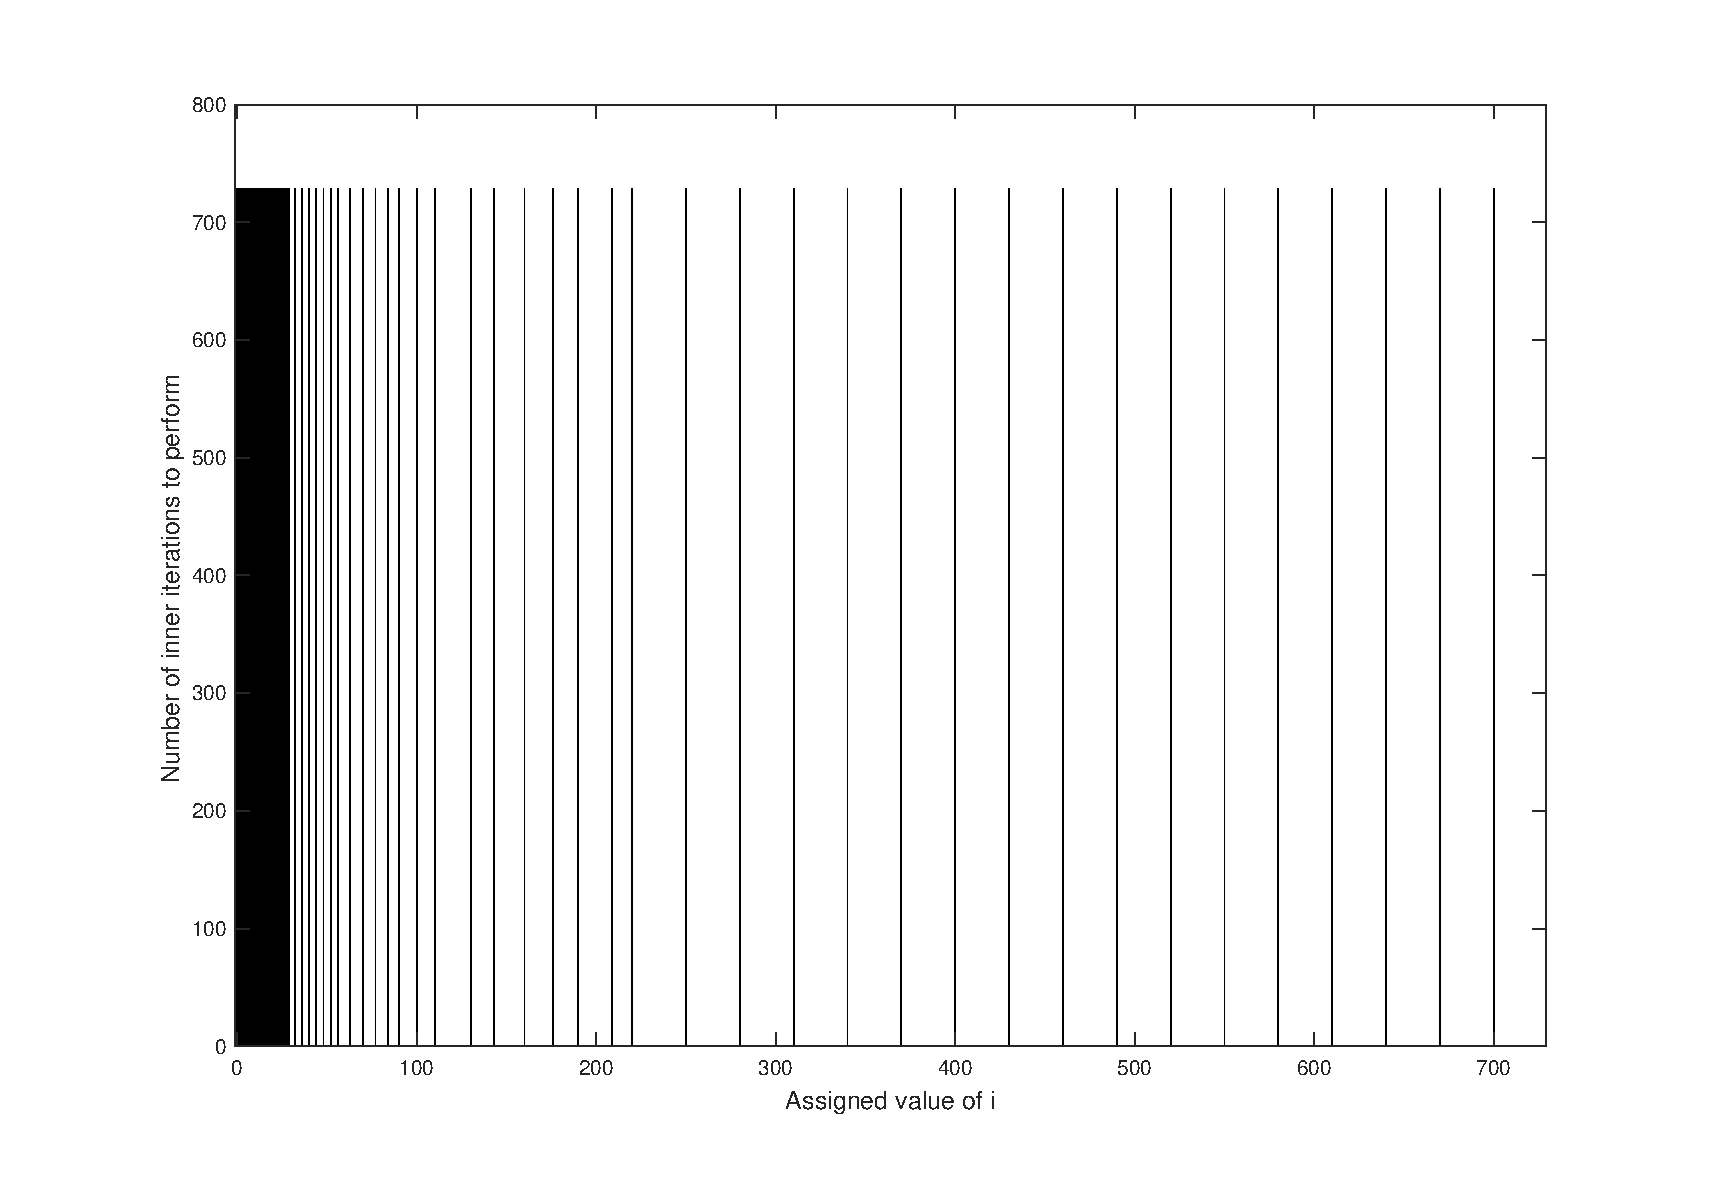
\includegraphics[height=.35\textheight]{part1_plots/loop2_balancing.eps}

% \end{figure}

\begin{figure}
    \begin{lstlisting}
        do i = 1,N

            do j = 1, jmax(i) 
        
                do k = 1,j 
                    
                    c(i) = c(i) + k * log(b(j,i)) * rN2
                
                end do
            
            end do
     
        end do
    \end{lstlisting}
    \caption{Loop 2; note that this loop is poorly-balanced as a result of the inner loop being iterated to either $1$ or $N$, depending on the value of \texttt{i}.}
    \label{listing:loop2}
\end{figure}

The results for Loop 1 are given in Figure \ref{fig:loop1results}. Clearly, the \tp{AUTO} scheduling performs worse than the serial case (note that, while the AUTO execution time has been extended across all chunk sizes, the chunk size was not specified and this has been done for clarity only.)
It is not immediately clear why this scheduling option performs this poorly, as there is no transparency in the scheduling implemented, but it is clear that this option should be avoided.

The performance of the \tp{STATIC, \textit{n}} scheduling routine decreases with increases in chunk size.
This is to be expected, and highlights the differences in balance in the loop; when contiguous chunks of $n$ iterations are distributed, the first threads will always perform more work than the final threads as a result of the work distribution for Loop 1.
For low chunk sizes, the high-work loops are relatively well-distributed amongst all threads, and thus there is relatively little idling and generally decreased performance time.
However, when high chunk sizes are used, the first thread takes the majority of the work, and thus acts as a bottleneck for the program execution: the higher the chunk size, the longer the final threads are idling waiting for the first thread(s) to finish.

This is readily seen from the profiling of the \tp{STATIC} scheduling option for chunk sizes of 1 and 64, respectively (Table \ref{tbl:loop1profiling}), where the work done by all threads for \tp{STATIC,1} is far higher than for \tp{STATIC,64}.

This also explains the behaviour of the \tp{STATIC} algorithms for the case where there's no chunk-size specified.
In this case, the chunk-size defaults to the ratio of the number of iterations to the number of threads.
The poorly-balanced first thread will thus act as a bottleneck here.

\begin{table}[b]
    \centering
    \begin{tabular}{@{}lllllll@{}}
    \toprule
    \multirow{2}{*}{\textbf{Thread number}} & \multicolumn{6}{c}{\textbf{Loading}}                \\
                                            & S,1    & S,64   & G,1    & G,64   & D,1    & D,64   \\ \midrule
    0                                       & 100\%  & 100\%  & 100\%  & 100\%  & 100\%  & 100\%  \\
    1                                       & 85.3\% & 57.7\% & 55.4\% & 55.5\% & 32.0\% & 57.9\% \\
    2                                       & 85.3\% & 57.7\% & 55.0\% & 55.5\% & 32.0\% & 57.9\% \\
    3                                       & 82.4\% & 57.7\% & 55.0\% & 55.5\% & 32.0\% & 57.9\% \\
    4                                       & 82.4\% & 57.6\% & 55.0\% & 55.5\% & 32.0\% & 57.8\% \\
    5                                       & 82.4\% & 57.6\% & 55.0\% & 55.5\% & 32.0\% & 57.8\% \\ \bottomrule
    \end{tabular}
    \caption{Loop 1 load balancing on each thread, reported from the Cray profiler. As expected, \tp{STATIC,64} has poorer load imbalance than \tp{STATIC,1}, but \tp{DYNAMIC,64} has better balancing than \tp{DYNAMIC,1}.}
    \label{tbl:loop1profiling}
\end{table}

As expected, \tp{DYNAMIC} and \tp{GUIDED} perform well for this loop.
Since \tp{DYNAMIC} assigns chunks of loop iterations to threads on a first-come, first-served basis, at small chunk sizes threads which are initially assigned less work will be assigned more work whilst other threads are still computing. 
\tp{GUIDED} functions similarly, but the loop iterations start off large and get expontentially smaller: thus, for loops with initially high amounts of work, such as this, we would expect good performance.

\begin{figure}
    \centering
    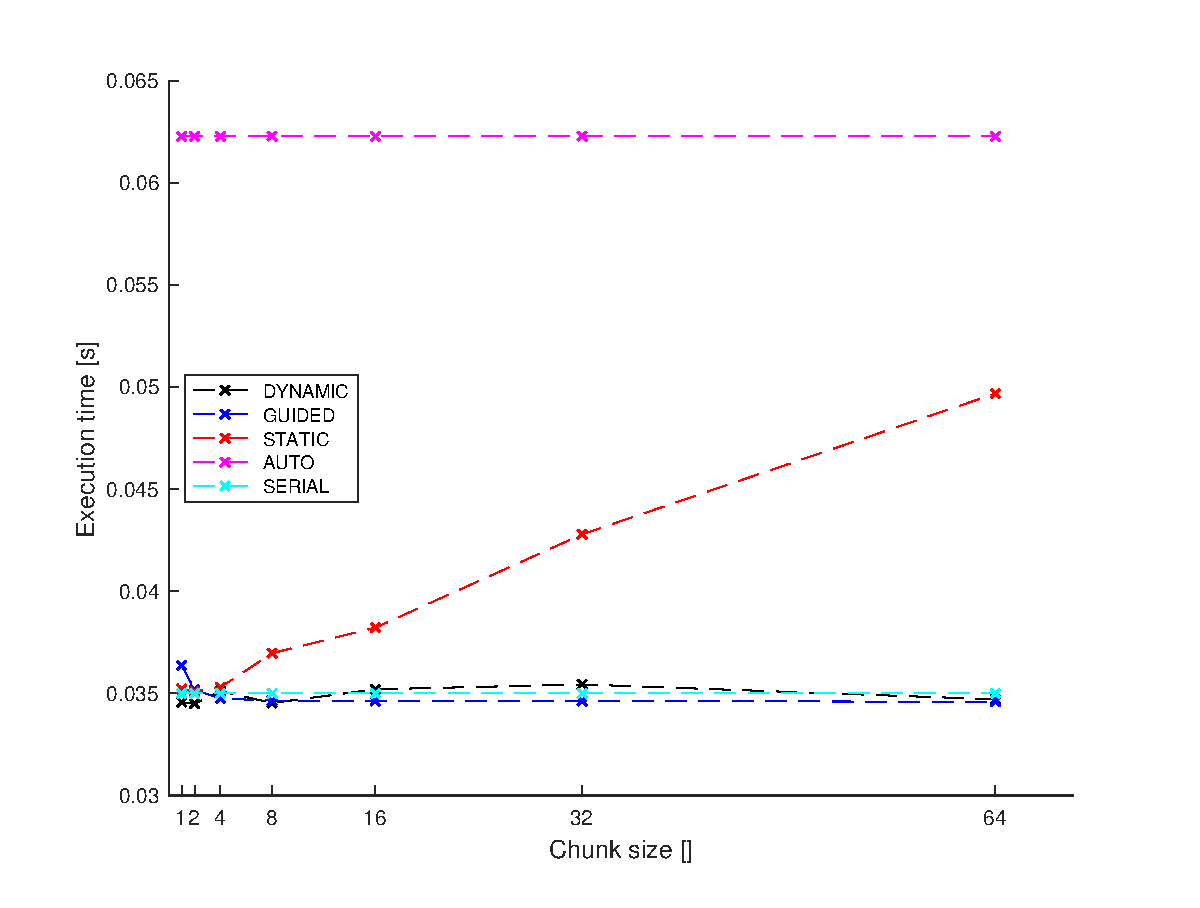
\includegraphics[height=.35\textheight]{part1_plots/all_part1.eps}
    \caption{Loop 1 execution performance for different scheduling algorithms: \tp{GUIDED,\textit{2}} provides the best performance here overall, but \tp{DYNAMIC} performs better across a wider range of chunk sizes.}
    \label{fig:loop1results}
\end{figure} 

\tp{GUIDED,2} produces the best performance for this problem, but not by any considerable margin.
It provides the best overall execution time of $0.03449$s, but this is only $.23\%$ above the average performance of the \tp{DYNAMIC} method. 
In fact, \tp{DYNAMIC} has generally superior performance at most chunk sizes when compared to \tp{GUIDED}, and helps to smooth the slight imbalance in the loops to maximise performance.
Therefore, while \tp{GUIDED,2} is the fastest scheduling choice here, \tp{DYNAMIC} may prove to be more versatile across a wider range of chunk sizes.

Also note that the performance of most of the routines with chunk size $1$ is also worse than the serial version, highlighting the scheduling overheads of OpenMP.

The results are relatively similar for Loop 2, and are provided in Figure \ref{fig:loop2results}. 

Again, the \tp{AUTO} scheduling performs poorly, and routines with chunk size $1$ perform worse than the serial case.

Because of the unusual loading in this loop, the first 30 iterations are required to do the maximum amount of work.
Therefore, scheduling algorithms that spread this initial work out across threads would reduce idling times for the unloading threads and thus increase performance.
This explains the behaviour of many of the scheduling algorithms above: when the chunk size begins to increase -- in the case of \tp{DYNAMIC} and \tp{GUIDED}, the minimum chunk size -- then fewer threads get assigned the initial amounts of work, and thus execution times will rise.

\begin{figure}
    \centering
    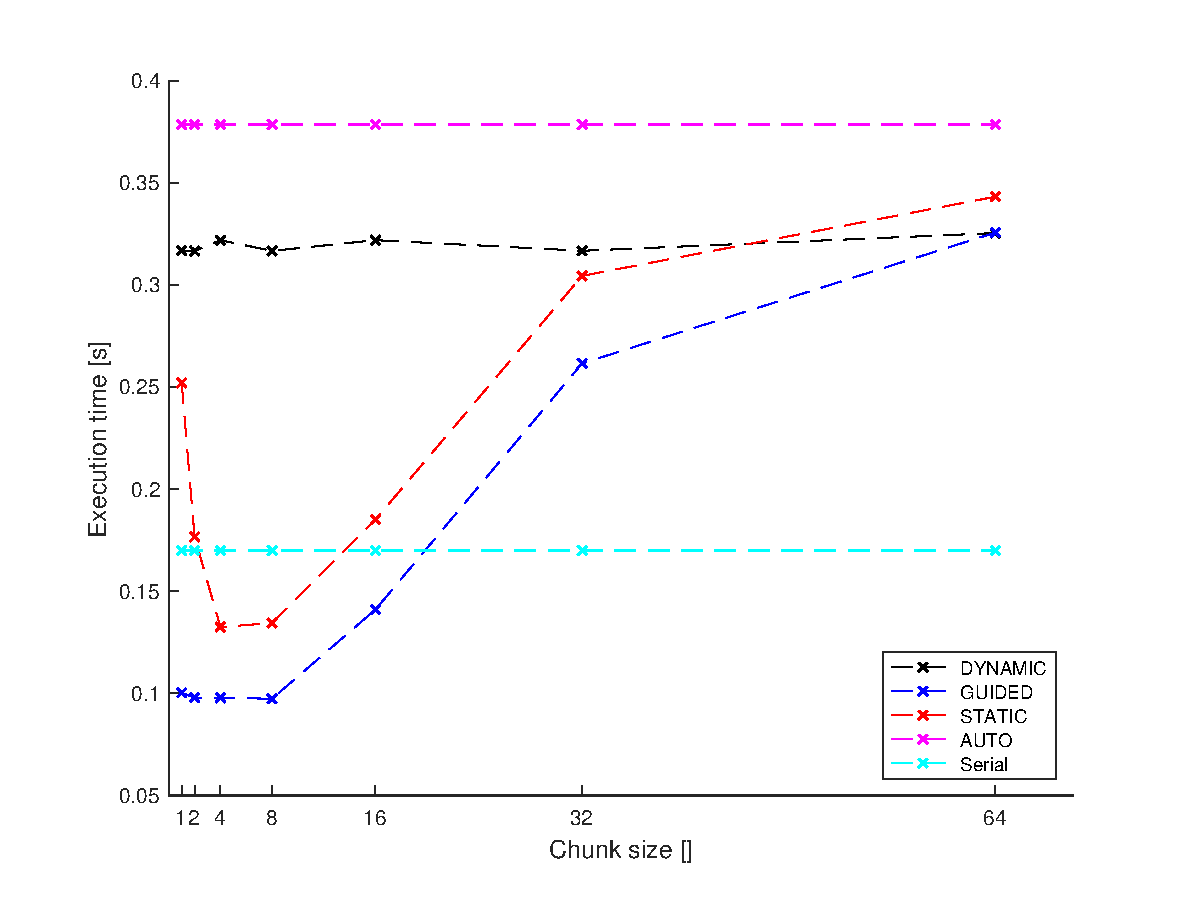
\includegraphics[height=.35\textheight]{part1_plots/all_part2.eps}
    \caption{Loop 2 execution performance for different scheduling algorithm. \tp{DYNAMIC,8} provides the best performance for Loop 2, but performance generally reduces with increasing chunk size.
    This is a quirk of the unusual loading for Loop 2.}
    \label{fig:loop2results}
\end{figure}

Interestingly, \tp{GUIDED} has constant performance for all chunk sizes.
This may suggest that only large chunk-sizes are being used in the algorithm, since the chunk size passed to the program specifies only the minimum chunks. 
Indeed, referring again to \ref{tbl:loop1profiling}, the loading profile for all threads changes only very slightly for the extrema of the chunk-sizes used.

\tp{DYNAMIC}, and specifically \tp{DYNAMIC,8}, has the best execution time for this problem. This is again expected, with \tp{DYNAMIC} allowing threads with low amounts of work to accept more.

\section*{OpenMP-standard Scheduling: Thread numbers}

Now we have determined the `best' scheduling options for each loop, we may investigate their thread-scaling.
Ideally, we would experience a true linear scaling, where the execution time decreases as a linear function of the number of threads used.
However, consider Amdahl's Law, which is often-cited in parallel computing:

$$
\text{Speedup}(s) = \frac{1}{\left( 1 - p\right) + \frac{p}{s}}
$$

which gives the factor of speedup, where $s$ represents the local speedup -- say, by parallelising -- and $p$ represents the amount of the program that is available to be parallelised.
Amdahl's Law provides a good metric for determining the maximum speedup we can expect from a parallel program, and provides the deduction that speeding up programs by using parallelism will be limited by our serial regions. 
In general, our processor efficiency -- how well we are using all our threads -- is a major limitation on program runtime.

As a result, it is rare (or near impossible) to see true linear scaling; even for a program that has 95\% of its code base eligible to be paralellised, speed-up will never exceed a factor of 20, no matter how many threads are used.

\begin{figure}
    \centering
    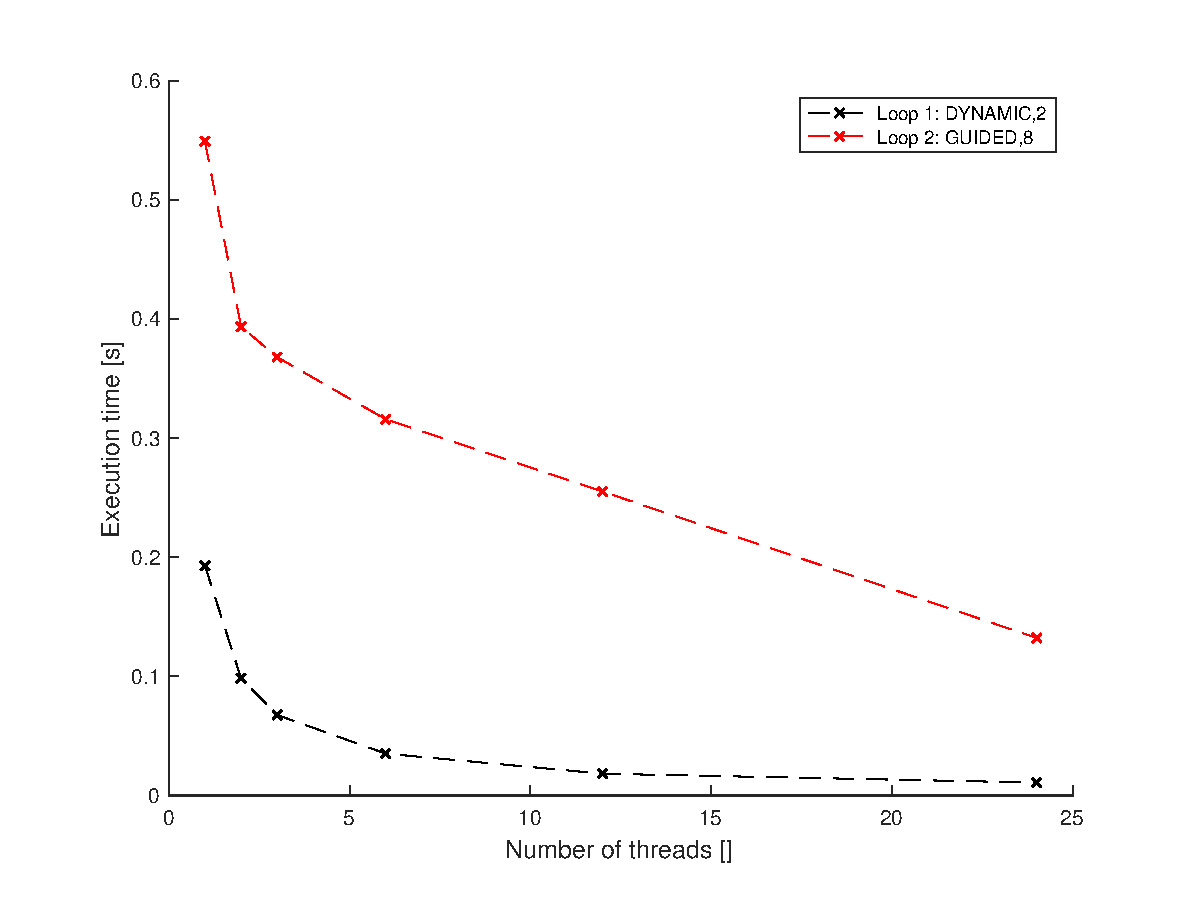
\includegraphics[height=.35\textheight]{part1_plots/bestruns_all}
    \caption{Loop execution times with respect to the number of threads used; we do not obtain linear scaling here, as a result of OpenMP overheads, but we do see a general increase in performance with thread numbers, as expected.}
    \label{fig:threadall}
\end{figure}

Figure \ref{fig:threadall} provides the speedup for both loops as the number of threads is varied.
It's immediately obvious that program execution times decrease with increasing thread numbers, as expected.

However, the scaling is generally poor, even despite the relatively large amount of parallelisable source code (recall that we are timing only the loop execution).
Loop 1's scaling factor is $0.7332$ per additional thread, and Loop 2 $0.1233$. 

\begin{figure}
    \centering
    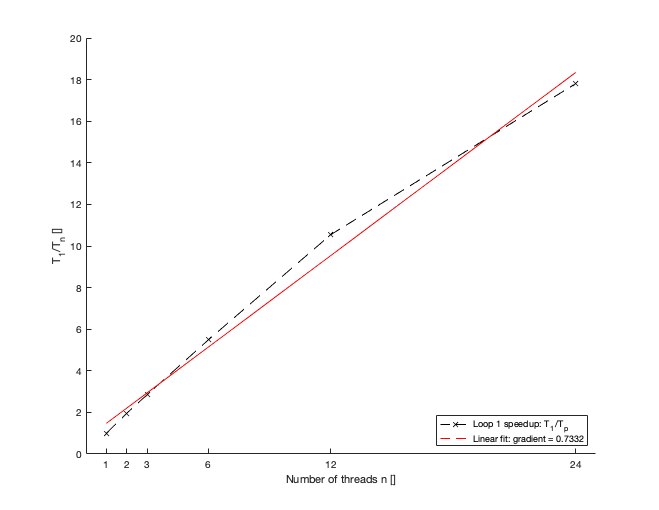
\includegraphics[height=.35\textheight]{part1_plots/loop1_speedup.png}
    \caption{The speedup for Loop 1 compared to the serial execution times. For low thread numbers, the scheduling overhead is not overcome, and performance suffers.}
    \label{fig:loop1speedup}
\end{figure}

There are several reasons why this performance is lower than the theory predicts. 
For Loop 1 (Figure \ref{fig:loop1speedup}), the optimal scheduling configuration has a low chunk-size, which is likely to incur significant scheduling overheads.
Similarly, while the loop is only mildly imbalanced, we are also expecting some communication overhead when threads are reassigned work and the data must be moved in memory.

For Loop 2 (Figure \ref{fig:loop2speedup}), the scaling is generally much worse.
Much of this, as discussed previously, will be due to synchronisation overheads when threads are kept working, and the extra few high-work iterations spaced evenly through the runtime will prevent threads becoming available.
Other overheads, such as communication overheads, will also be present, but dominated by the synchronisation overheads.

\section*{Affinity Scheduling}

In view of the performance of the OpenMP-standard loops, attention now turns to an implementation of static partitioned affinity scheduling, an algorithm developed by \citet{273046}.
The algorithm is designed for parallel loops nested inside serial loops, and aims to ensure that cache misses and processor idling times are minimised.

The algorithm functions by allocating an equal proportion of the total work to each thread. 
When a thread finishes each of its initial allocation, it will `steal' work from the thread with the most remaining of its initial allocation.

\begin{figure}
    \centering
    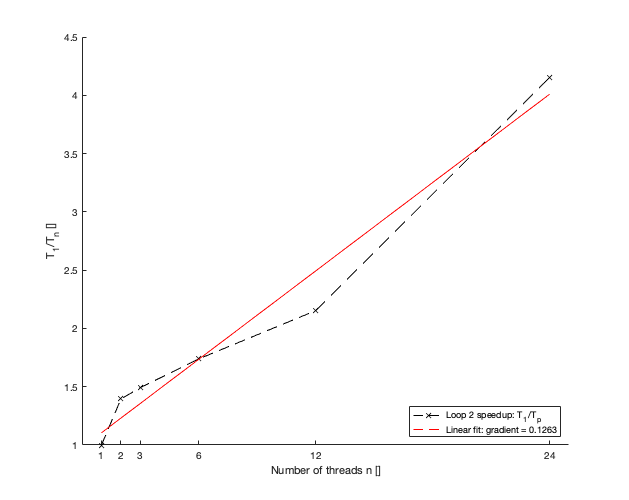
\includegraphics[height=.35\textheight]{part1_plots/loop2_speedup.png}
    \caption{The speedup for Loop 2 compared to the serial execution times. The scaling here is poor as a result of the loading keeping threads working when they would otherwise be idle.}
    \label{fig:loop2speedup}
\end{figure}

Much of the algorithm's speed comes from the determinstic loop allocation at the initial execution of the loop, which ensures that the $i$th processor holds the $i$th chunk of iterations.
By doing so, the data required for repeated executions of the loop will already be stored in cache, removing the need for relatively expensive memory movements.
Also, the algorithm assumes, at first, that the loop is perfectly balanced, and therefore takes initially large chunks of work.
Thus, there is only a scheduling overhead at the beginning of the loop.

When each thread does finish its local thread, work is reassigned to smooth the load imbalance and prevent threads from idling.
By only reassigning at the point of imbalance, unlike \tp{DYNAMIC} or \tp{GUIDED} which begin to perform large re-scheduling in the latter portions of the loop, the scheduling and memory re-allocation overhead is only incurred when required, and memory is moved at most twice when work is reallocated.

\subsection*{Implementation}

A description the algorithms' implementation follows:

Each thread is initially assigned $P/N$ iterations, where $P$ is the total number of iterations and $N$ the number of threads. 
Should $N$ not divide evenly into $P$, then the remainder $r$ is scattered across the first $r$ threads.
The number of iterations each thread is to perform is stored in an array indexed by the thread identifier retrieved from \tp{OMP\_GET\_THREAD\_NUM}.
Since this array must be shared in the parallel region, the synchronisation of, and access to, the array must be closely controlled.
\tp{CRITICAL} sections or \tp{LOCK}s must be implemented to prevent race conditions and unintended overwrites:
a discussion on this is given later.
If \tp{LOCK}s are used, another array is created that holds the lock from every thread, indexed by the thread identification number.

Other variables, such as the number of threads, and the value of $P/N$, are also shared.
By default, all other variables are scoped as \tp{PRIVATE} in all parallel regions.

At this point, each thread is begins work on $1/P$ iterations of its initial assignment, and updates the (shared) number of iterations array to announce to the other threads that it has taken those iterations to be executed.
This contiguous assignment ensures that repeated iterations will access data already stored in local caches.

This assignment is again enclosed in either a \tp{CRITICAL} region, or \tp{LOCK}s are used to prevent race conditions on each element of the array.
From here forwards, the number of iterations array tracks the number of iterations remaining for each thread.

The upper and lower bounds of iteration counter are then determined parametrically from the thread identification number and the number of iterations remaining; the algorithm starts at the `bottom' of each thread's chunk and moves upward.

In order to aid the execution of this type of scheduling algorithm, the \tp{loop1} and \tp{loop2} subroutines now take in two \tp{integer}-type arguments, that set the upper and lower bounds for the outer loop.
Owing to the variable scoping in the internal procedures in Fortran, the shared arrays \tp{a}, \tp{b} and \tp{c} may be accessed without specification of their OpenMP scope.

\begin{figure}
    \centering
    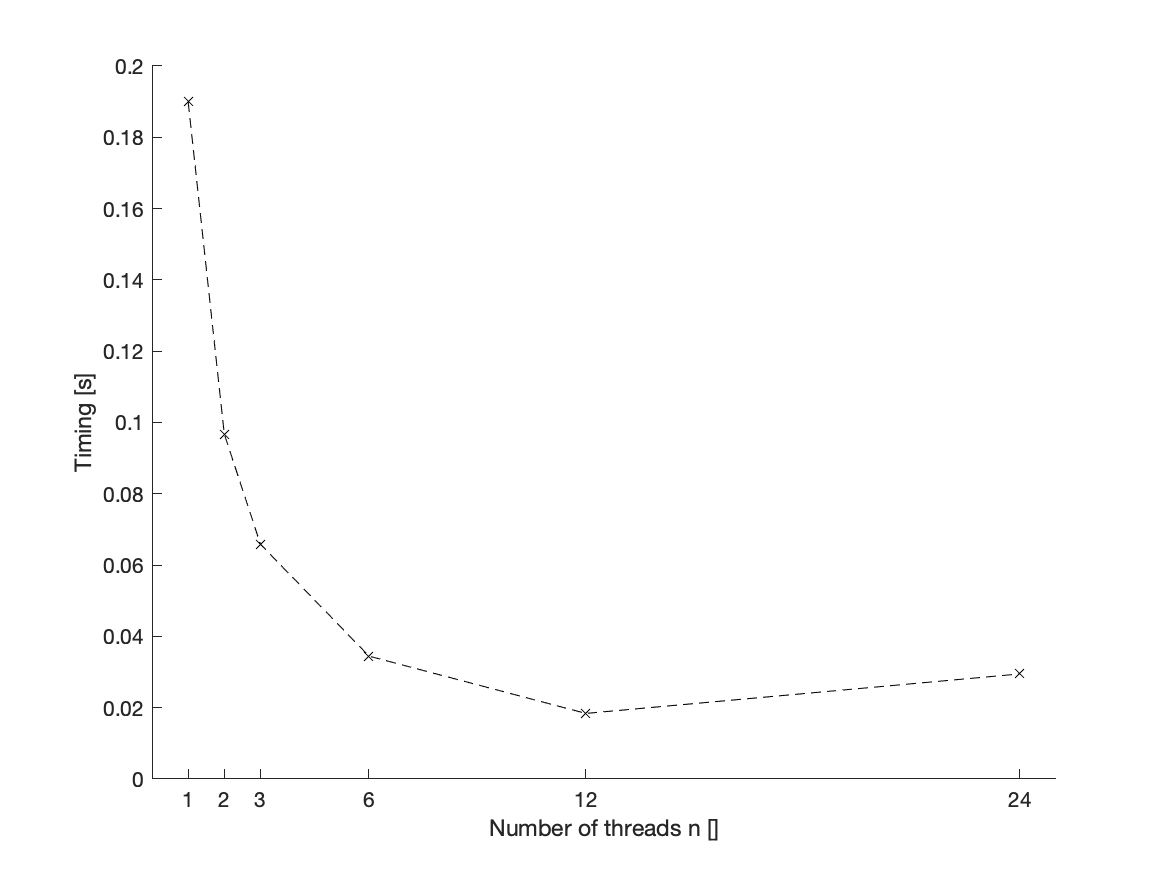
\includegraphics[height=.3\textheight]{part2_plots/affinity_loop1}
    \caption{Execution times for Loop 1, scheduled using the static partitioned affinity scheduling algorithm. We obtain better performance as we increase the number of threads, until the array chunks no longer fit in the processor cache.}
    \label{fig:affinityloop1}
\end{figure}

This process is repeated for all threads until one or more completes its initial assignment of threads.
At this point, it is likely, especially in imbalanced loops, that other threads will still be working.
So as to minimise idling times, each `finished' processor -- that is, one that has completed its initial assignment -- will use the array of remaining iterations to determine which other thread is currently the most loaded.
The finished thread will then `steal' work from the most loaded thread, appropriately emunlating the thread identifiers of the most loaded thread to properly update the shared arrays to announce to other threads that it has taken some of the loaded thread's iterations to be executed.
So that no two finished threads are assigned the same work, \tp{CRITICAL}s or \tp{LOCK}s are used again.

When all threads have finished their local assignment, the loop has completed.

\subsection*{Results: Affinity Scheduling}

The results for Loop 1 using affinity scheduling are presented in Figure \ref{fig:affinityloop1}. 
For the equivalent number of threads as the scheduling methods visited earlier (6), performance is marginally better, with a performance increase of 10\textsuperscript{-4}; however, performance with respect to the OpenMP-standard scheduling algorithms decreases as the number of threads increases.

\begin{figure}
    \centering
    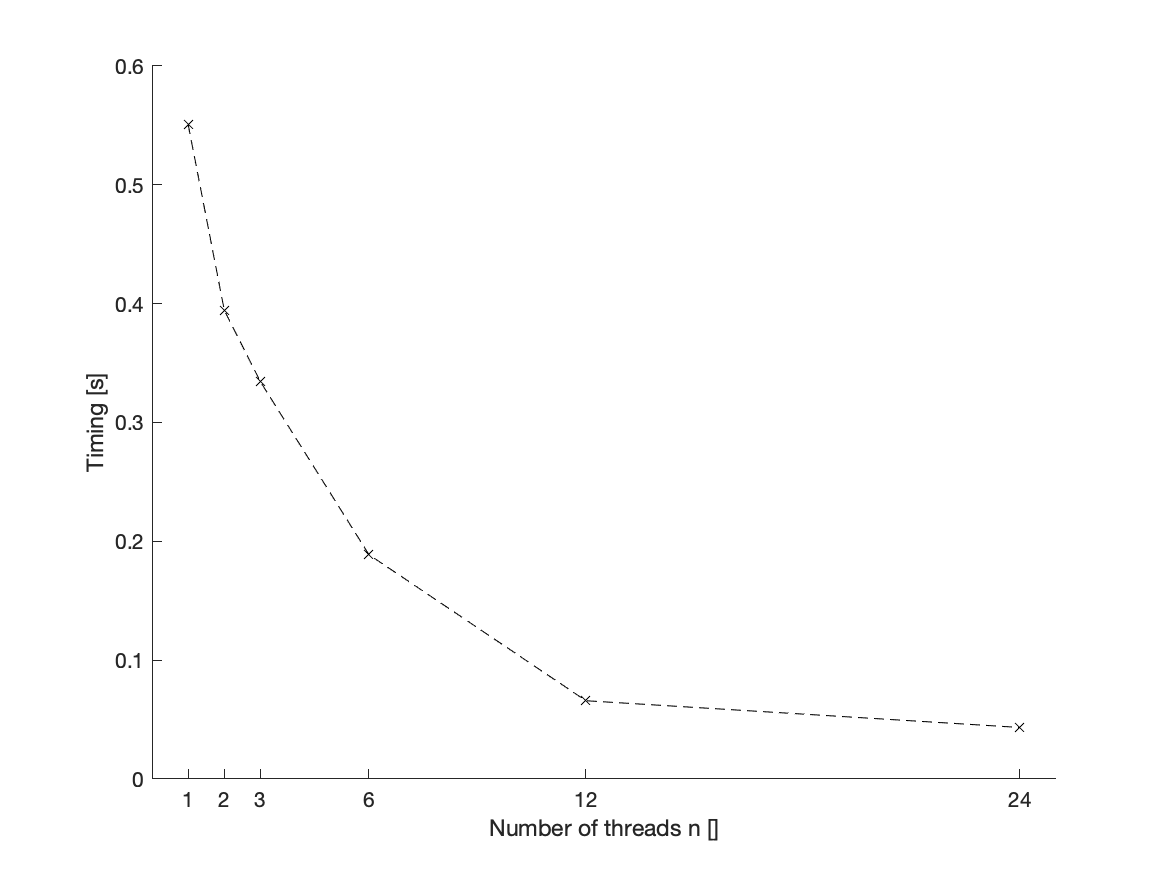
\includegraphics[height=.35\textheight]{part2_plots/affinity_loop2}
    \caption{Execution times for Loop 2, scheduled using the static partitioned affinity scheduling algorithm. Again, we obtain better performance as we increase the number of threads, although the performance does not scale one-to-one with the number of threads.}
    \label{fig:affinityloop2}
\end{figure}

The increase in performance for moderate thread numbers is to be expected.
The initial, large deterministic assignment of iterations to each thread ensures that each thread stores the data it requires in cache.
While the \tp{DYNAMIC} and \tp{GUIDED} systems also perform an initially large assignment of iterations, there is no guarantee that it is deterministic.

The load balancing is also only performed when required when using affinity scheduling, whereas \tp{GUIDED} and \tp{DYNAMIC} will perform reassignments -- and thus incur communication and synchronisation overheads -- regardless of the load balancing.
When profiling, the OpenMP overheads are indeed seen to be lower.

The performance also scales well with the number of threads, with an increase in speedup ratio of approximately $0.8$ per additional thread: much of the reasoning behind this has been discussed previously.

When compared with the best Open-MP standard scheduling algorithms, affinity struggles at high thread numbers.
Much of this is as a by-product of the synchronisation constructs used to protect the shared iteration arrays: at large thread numbers, threads will spend a significant amount of time waiting for data to be made available.
Profiling the parallel code reveals that up to $5$\% of total program runtime is as a result of these synchronisation overheads.

We also notice a decrease in performance for 24 threads when referring to Figure \ref{fig:loop1speedup}, which provides the ratio of serial execution time to parallel execution time for Loop 1.
While the exact reason for this is unclear, consider the following:

\begin{figure}
    \centering
    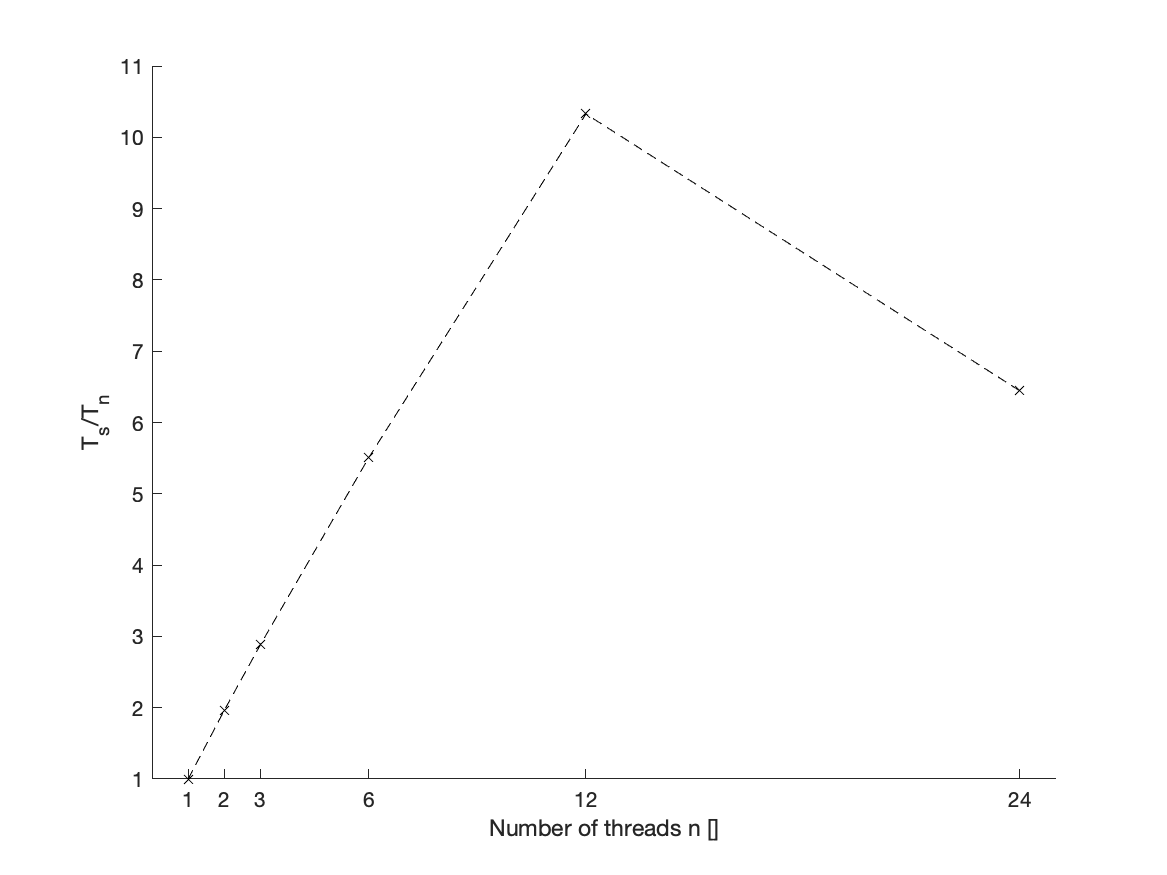
\includegraphics[height=.35\textheight]{part2_plots/speedup_affinity_loop1.png}
    \caption{The ratio of execution time using $n$ threads to serial execution time for Loop 1; the drop in performance at 24 threads could be as a result of data no longer fitting in the cache.}
\end{figure}

Each processor on the ARCHER system (Intel® Xeon® Processor E5-2697 v2\footnote{\href{http://archer.ac.uk/about-archer/hardware/}{ARCHER: Hardware}}) has a 30MB cache\footnote{\href{https://ark.intel.com/content/www/us/en/ark/products/75283/intel-xeon-processor-e5-2697-v2-30m-cache-2-70-ghz.html}{Intel Xeon E5-2697-V2}}.
The data arrays \tp{a} and \tp{b} are 4-byte \tp{REAL}-type arrays, and are both square arrays of 729 elements.
A quick estimate of the memory size of this array yields $2 \times 729 \times 729 \times 4 \text{bytes} = 4.251\text{MB}$ in the data arrays alone.
In shared memory systems, the cache is shared between every thread, and thus at 24 threads, each thread may have at most 1.25MB of local cache memory.
It could be, therefore, that the data lines for the array does not fit in the processor cache effectively at 24 threads, and thus the communication overhead is reducing the run-time.
Interestingly, profiling the program shows a total memory usage of 191MB, which provides some evidence to this theory.
Considering we're dealing with otherwise very quick execution times, this overhead could be significant, although this drop in performance wasn't encountered in the OpenMP-standard routines.

Alternatively, the reduction in performance could be due to competition between threads during the work (re-)assignment phases.

\begin{figure}
    \centering
    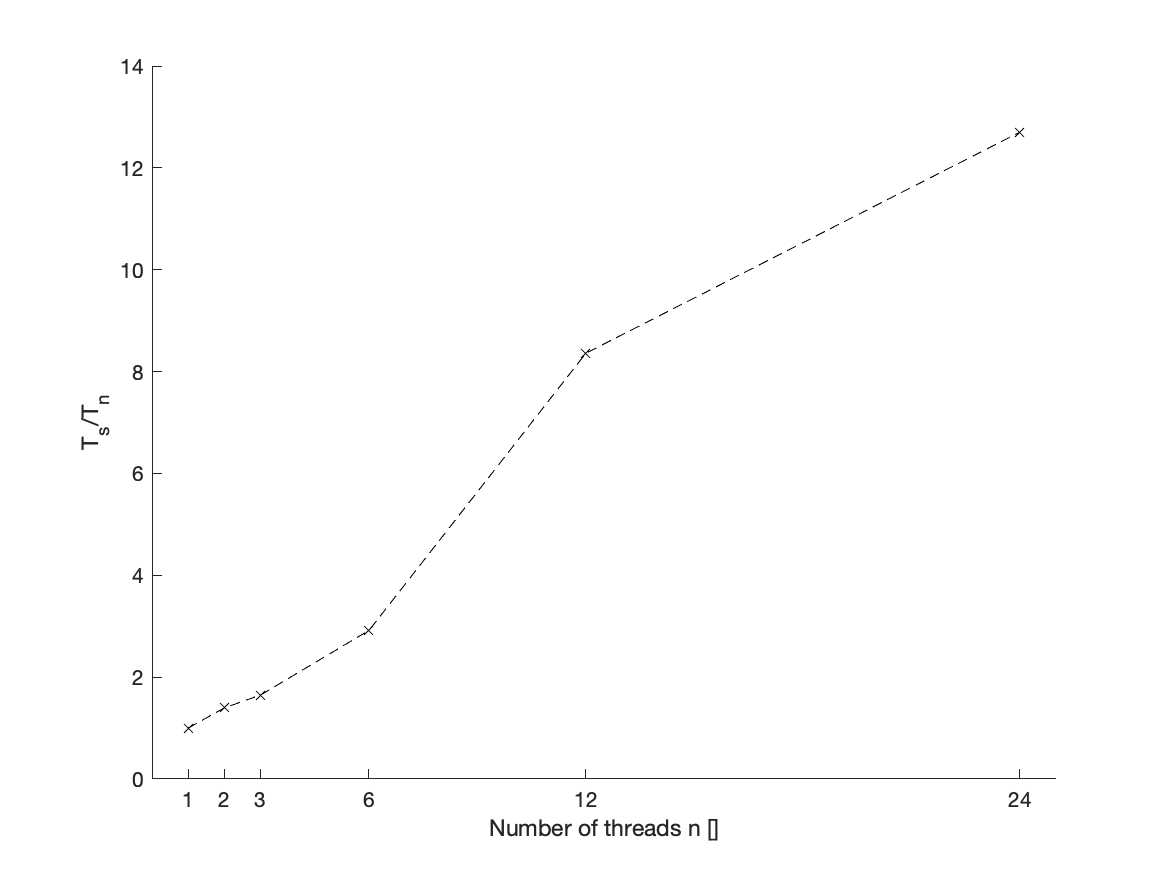
\includegraphics[height=.35\textheight]{part2_plots/speedup_affinity_loop2.png}
    \caption{The ratio of execution time using $n$ threads to serial execution time for Loop 2; we note a poorer scaling than for Loop 1, but much of this is as a result of poor load balancing and the associated synchronisation overheads.}
\end{figure}

The results for Loop 2 are presented in Figure \ref{fig:affinityloop2}.
Performance at all thread numbers is superior when compared to the OpenMP-standard schedulers;
it's likely that the decrease in execution time is as a result of a better load balancing scheme.

The scaling is generally much poorer here, at approximately $0.54$, but this is still better than the scaling for the standard algorithms.
For a less balanced loop, it's likely that the overheads due to communication -- with the data arrays again occupying a large amount of space in cache, at 2.12MB -- are dwarfed by synchronisation and load balancing overheads: in fact, the profiler reports that 10.9\% of the total program execution is spent on the \tp{CRITICAL} and \tp{LOCK} sections for Loop 2.

\subsection*{\tp{CRITICAL} vs. \tp{LOCK}s}\label{s:locks}

There are two methods of general synchronisation defined in the OpenMP standard: \tp{CRITICAL} and \tp{LOCK}s. 
\tp{CRITICAL} may be thought of as protecting code sections: regions may only be entered by one thread at a time, and thus there is a significant synchronisation overhead whilst threads are waiting to enter the \tp{CRITICAL} region.
\tp{LOCK}s act on data, and restrict access to certain parts of data when a thread `locks' or `unlocks' a portion of the data.


\begin{figure}
    \centering
    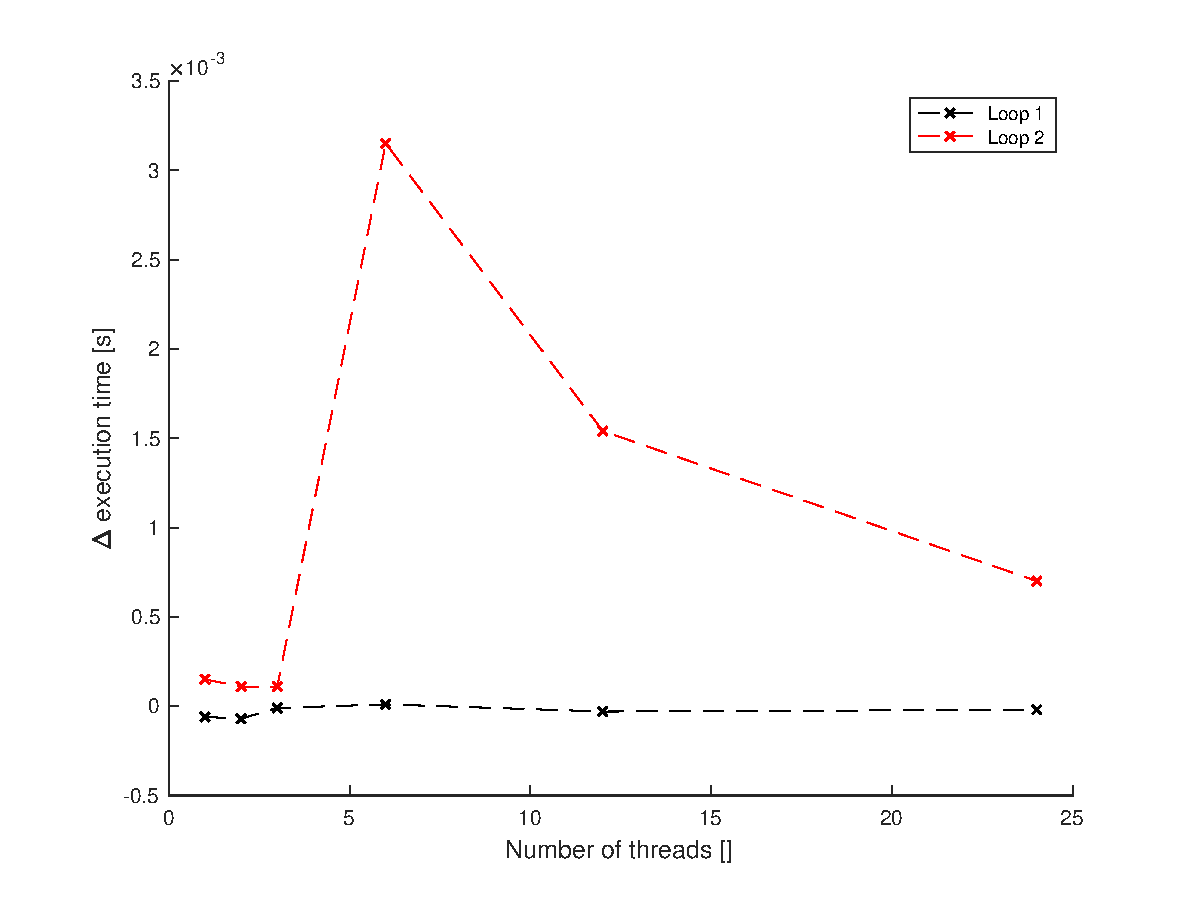
\includegraphics[height=.35\textheight]{part2_plots/criticalvslock}
    \caption{The change in execution time when using critical regions, as compared to locks; locks are found to be faster by approximately 10\%.}
    \label{fig:criticalvslock}
\end{figure}

Two versions of the affinity scheduling algorithms were implemented: one using critical regions, and another using locks.
By doing so, the best-performing implementation could be selected for timing, and the impact on speed investigated.

The results of this investigation are presented in Figure \ref{fig:criticalvslock}. 
It is found that, for Loop 1, the differences are negligible, and for Loop 2 the differences are up to 10\% in run time.
This may suggest that the original \tp{CRITICAL} regions in Loop 1 were unlikely to hinder run time, implying that the amount of time threads spend doing work compared to assigning work, is low.

Alternatively, for Loop 2, preventing threads from iterating at the start of a \tp{CRITICAL} region appears to be a large bottleneck in program execution.

Such timings or profilings would need to be performed to ascertain the impact of either synchronisation structure on the program.
In general, where \tp{CRITICAL} regions reduce performance, they are far easier to implement.
For large code bases, it may be a trade-off between programming time and execution time.

\section*{Limitations}

The study presented in this work has limitations that should be acknowledged when considering the results.

Firstly, and perhaps most importantly, the execution times in this study are very small, with the lowest being $0.019$s for 100 repetitions of the loop being parallelised.
At such small run times, the program will be dominated by the (serial) overheads of OpenMP, at which point the increase in loop execution performance is diminished.
As discussed previously, these overheads were reported to be up to $7\%$ during profiling. 

Furthermore, at these small run times, the effect of variable compute performance is exacerbated. 
While every attempt was made to attempt to ensure all jobs were run on the same node -- by submitting all jobs as a batch and adjusted using environment variables -- some variable performance is possible, although averages of several run times were used.
In particular, the profiling was performed separate to the main set of runs.

Also, traditional scientific codes typically use double-precision \tp{REAL}s, where these loops use single-precision \tp{REAL}s.
Representing numbers in double-precision incurs a performance overhead:
When using the \tp{-s real64} flag with the Cray Fortran compiler on ARCHER, the loop execution times increase by approximately 10\textsuperscript{-3}.
Given that execution times are on the order of 10\textsuperscript{-2}, this difference may be significant.

This study also only concerns itself with the performance gain from implementing OpenMP.
While speedups of a factor of 12 are made here, the implementation time is several hours.
Thus, in general production codes, the time spent on parallelising the loops must be justified by the increase in performance.

\begin{itemize}
    \item Variable node performance
    \item We're running for 0.3 seconds - how much speedup are we actually going to get? repeat over 1000 iterations maybe?
    \item This is an exemplar problem, and is not massively practical. Also a very small code base - practicality of having arrays be smol?
    \item Easy to implement - miss out the `development time' costs 
\end{itemize}

\section*{Conclusion}

This is some form of conclusion I'm making up on the spot

"Lorem ipsum dolor sit amet, consectetur adipiscing elit, sed do eiusmod tempor incididunt ut labore et dolore magna aliqua. Ut enim ad minim veniam, quis nostrud exercitation ullamco laboris nisi ut aliquip ex ea commodo consequat. Duis aute irure dolor in reprehenderit in voluptate velit esse cillum dolore eu fugiat nulla pariatur. Excepteur sint occaecat cupidatat non proident, sunt in culpa qui officia deserunt mollit anim id est laborum."

\bibliographystyle{plainnat}

\newpage
\bibliography{bib.bib}

\end{document}
